\section{Basis of Our Approach}
\label{sec:approach}

%Nevertheless, tools such as BLAST \cite{BLAST1990} and BWA-MEM \cite{BWA-MEM} use the customized versions of the S-W algorithms.
%In BWA-MEM, we have three important observations that prevent us from using conventional wavefront technique for hardware acceleration.
Our acceleration engine design is based on the following three important observations 
discovered from the analysis of the S-W code in BWA-MEM.
%%%From the observations, we find that the wavefront-based architectures are inefficient to be applied in BWA-MEM.
%%%
%%%For simplicity without losing generality, 
%%%we abstract the total resource of an acceleration platform into a given number of unified processing elements (PEs) for illustration. 
%%%We also assume that each PE is capable of producing one DP computation per cycle to fill the score matrix. 
%%%A \textit{kernel} is composed of a group of PEs and can be assigned to execute one S-W task.
%%%We denote $m$x$n$ as a pair of input strings for the S-W algorithm with length $m$ and $n$. 
%%%The maximum achievable degree of parallelism is bounded by the length of the shorter string.

\vspace{1pt}
\textbf{Observation 1: Enormous Task-Level Parallelism}
\vspace{1pt}

A sequencer can generate billions of reads from a single individual for analysis in today's NGS flow.
The trend is to increase both the number of reads and the size of each read for more accurate analysis.
Therefore, the significant amount of data generates enormous task-level parallelism, 
which makes us reexamine the conventional wavefront technique for accelerating the S-W algorithm.

Conventional wavefront techniques exploit the inner-task anti-diagonal parallelism to maxmize the speedup for a single task.
However, the wavefront implementation is not optimal when the task-level parallelism is several orders of magnitude larger than the inner-task parallelism.
This is because the resources for implementing accelerators is limited.
We have to decide if the resource should be used for exploiting task-level parallelism or inner-task parallelism.
This influences the dynamic PE utilization rate, i.e. the throughput, and thus has a strong impact on performance.

%%%The three designs listed in Table \ref{tab:example} are used to demonstrate the performance impact on low PE utilization.
%%%We use 40 12x50 S-W tasks as input.
%%%Both Design 1 and Design 2 use the wavefront technique, which has multiple PEs in one kernel, 
%%%in order to exploit the inner-task parallelism.
%%%Design 3 has the maximum number of kernels and can fully exploit the task-level parallelism.
%%%With the same number of PEs, Design 3 outperforms the others since its PEs are fully utilized all the time.
%%%For Design 1, the maximum degree parallelism is 12, which is not divisible by the number of PEs per kernel (8).
%%%Therefore, some of the PEs are not fully utilized and it leads to poor performance.
%%%
%%%\input TBL/example
%%%
\vspace{1pt}
\textbf{Observation 2: Significantly Varied-Size Inputs}
\vspace{1pt}

The sharply varied input sizes of S-W in BWA-MEM results in a considerable waste of resources, i.e. low PE utilization, in wavefront-based designs. 
For example, a kernel of 10 PEs, fits perfectly for a 10x100 S-W task, but is only able to reach at most a 65\% resource utilization for a 13x103 input. 
This is because the length of the maximal anti-diagonals of the 13x103 input is 13, 
which is not divisible by the number of PEs in the kernel.
Figure \ref{fig:F4C2} provides a histogram of the sizes of the shorter strings (bounding the maximum degrees of parallelism) over 10M inputs of randomly selected BWA-MEM S-W tasks. 
The sizes range from one to 84, and none of them has more than 5\% of the 10M of inputs. 
This significant diversity of input sizes makes it prohibitive to choose one or a few kinds of PEs to avoid wasting of resources.
The only choice is to have each kernel only one PE, which means the anti-diagonal parallelism gets totally ignored.
%Assume that there is a kernel of 10 PEs to execute a 10x30 Smith-Waterman task. A 10x30 matrix has 39 anti-diagonal, each of which has at most 10 elements, so it takes 39 cycles for our 10-PE kernel to finish the task. However, the 10 PEs get fully utilized in only 21 cycles and the total PE utilization ratio is only 77\%, because of the filling and draining of the pipeline. The filling and draining inefficiency can be ignored if the input size is relatively large compared to the kernel size, e.g. a 10x10,000 task on a 10-PE kernel, but the inputs of BWA-MEM Smith-Waterman do not fall into this category. Figure \ref{fig:F4C2} provides a histogram of the lengths of the shorter strings (bounding the maximum degrees of parallelism) over 10 million randomly selected BWA-MEM Smith-Waterman tasks. The average length of the shorter strings is only 34 and approximately 25\% of the inputs has their shorter strings less than 10 in length. Configuring each kernel in a large size will surely lead to a low resource utilization rate in BWA-MEM.
\begin{figure}[!hbt]
	\begin{center}
		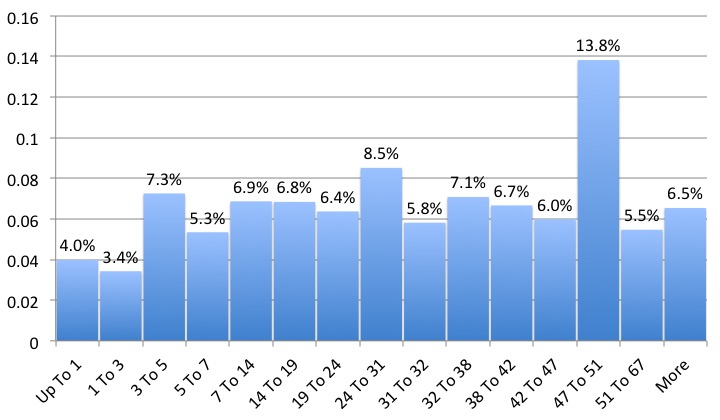
\includegraphics[width=3.2in]{Figures/Figure4C2.jpg}
		\caption {Histogram of the lengths of the shorter input strings collected from 10 million randomly selected BWA-MEM seed extension tasks. As is clearly illustrated in the histogram, the input sizes of the seed extension tasks in BWA-MEM are extremely heterogeneous, causing an inevitable waste of resources using wavefront-based designs.}
		\label{fig:F4C2}
	\end{center}
\end{figure}
%Another source of inadequate utilization comes from the irregular sizes of inputs. For a kernel of 10 PEs fed by a 13x37 Smith-Waterman task, the 13-element anti-diagonal has to consume 2 cycles, and the second cycle calculates only 3 elements, leaving 7 PEs unused and 65\% utilization rate in the two cycles. Admittedly, it has potential for the 10 PEs to calculate elements crossing anti-diagonals, but the control logic of each PE will consequently become much more complicated and take more area, which in turn decrease the number of PEs an accelerator platform can form. Based on our profiling over 10 million randomly selected tasks, the length of the shorter string ranges from 1 up to 84 consecutively, without any number showing up more than 5\%. Therefore, this kind of inefficient utilization is inevitable in BWA-MEM unless each kernel has only 1 PE.

\vspace{1pt}
\textbf{Observation 3: Pruning Strategies}
\vspace{1pt}

Derived from the X-dropoff pruning strategy in BLAST \cite{BLAST1990}, 
BWA-MEM's pruning strategy is able to save over 50\% in computation efforts for S-W tasks, as illustrated in Figure \ref{fig:F2C2}. 
%%%BWA-MEM's pruning strategy is able to save over 50\% in computation efforts for S-W tasks, as discussed in Section \ref{subsec:Smith-Waterman}. 
However, the pruning strategy destroys the basis of the anti-diagonal parallelism, as described in detail in \cite{BWA-MEM}, 
Moreover, the results generated by the extended S-W in BWA-MEM will be slightly different from those obtained by the standard S-W. 
This increases the difficulty of integrating existing wavefront-based works into BWA-MEM for verification concern. 
Even if the difficulty of integration can be overcome, 
the potential speedup from pruning would have to be sacrificed due to its incompatibility against the wavefront technique.
It will be even worse when the sizes of seeds becomes longer, which is the future trend for NGS.
%%%For Design 3 illustrated in Table \ref{tab:example}, it can be further accelerated by 2x with 50\% of computation pruned (1500 cycles). 
%%%However, the wavefront-based architectures, like Design 1 and 2, cannot leverage the benefits of pruning.
\begin{figure}[!hbt]
	\begin{center}
		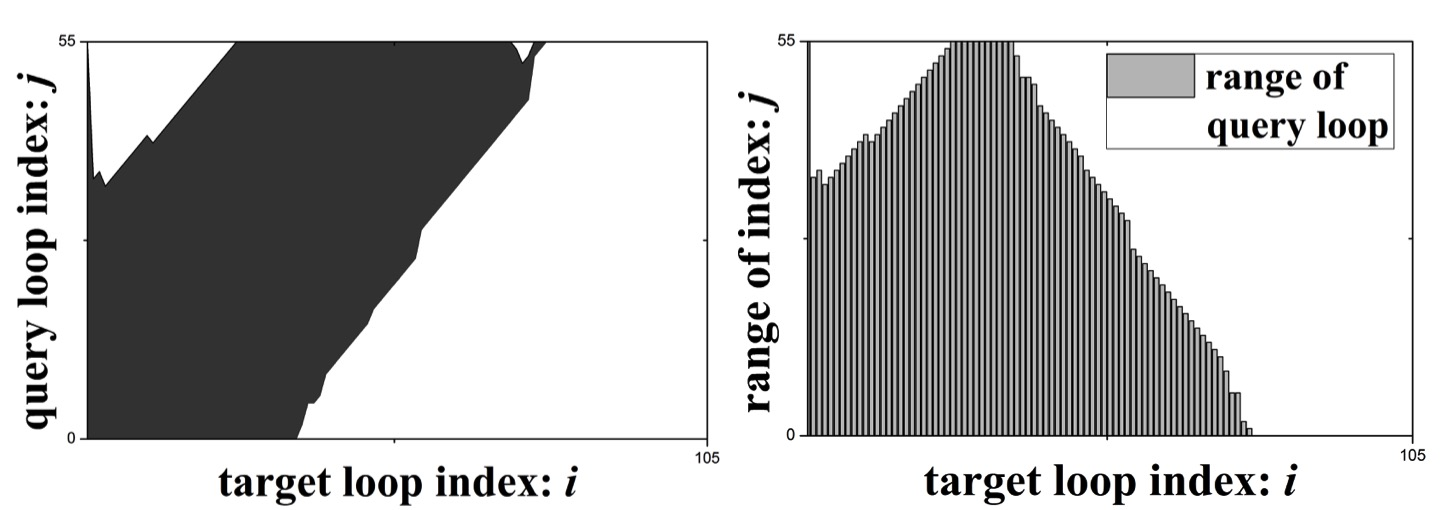
\includegraphics[width=3.2in]{Figures/Figure2C2.jpg}
		\caption {A 55x105 BWA-MEM Smith-Waterman task. The general S-W algorithm requires filling up a 55x105 matrix (5775 elements), but only 2836 elements (49\%) were actually filled with the help of pruning. The shaded area in the left graph illustrates the elements that got filled, and the right graph shows how many elements for each target loop index are actually calculated.}
		\label{fig:F2C2}
	\end{center}
\end{figure}
%\subsection{Simple is Best: A Motivational Example} 
%\label{subsec:motivation}

%The three key observations described in Section \ref{subsec:inefficiency} inspire us to develop a novel architecture 
%for the customized S-W algorithm to replace the traditional wavefront-based design. 
%Before we discuss the details of the architecture design, a motivational example is used to illustrate the inefficiency of wavefront technique.
%We assume that a given accelerator platform has eight PEs in total based on the resource constraint and is fed with 40 12x50 Smith-Waterman tasks. 
%We compare three design choices listed below.

%\vspace{1pt}
%\textit{Design 1: 1 kernel of 8 PEs}

%\vspace{1pt}
%\textit{Design 2: 2 kernels, 4 PEs per kernel}

%\vspace{1pt}
%\textit{Design 3: 8 kernels, 1 PE kernel}
%\vspace{1pt}

%Design 1 assigned all the resources to a single kernel and thus this kernel is the fastest kernel among all designs. 
%However, since the maximum degree of parallelism ($12$) is not divisible by the kernel size ($8$), some of the PEs are idled during computation. 
%The latency of each task and the total execution time is 106 and 4240 cycles, respectively.

%For Design 2, the PEs are almost fully utilized since the maximum degree of parallelism ($12$) is divisible by the kernel size ($4$). 
%The latency of each task and the total execution time is 159 and 3180 cycles, respectively.

%Design 3 reaches the other extreme by abandoning anti-diagonal parallelism. 
%Each kernel has the longest latency, 600 cycles, among all three designs. 
%However, Design 3 can achieve the maximum degree of task-level parallelism, and thus achieves the ideal 3000-cycle runtime.

%This example clearly demonstrates the design scheme that maximizes the number of simple kernels can lead to better performance
%when the task-level parallelism dominates.
%A wavefront-based kernel with multiple PEs reduces the latency of a task, but at the cost of low resource utilization. 
%It only works well when 1) the task-level parallelism is limited, or 2) the input size is homogeneous. 

%However, for BWA-MEM, the task-level parallelism is almost infinite as pointed out in Observation 1.
%Also, the input sizes of S-W tasks vary sharply as discussed in Observation 2. 
%In this case, the throughput becomes vital and the latency improvement by exploiting the inner-task parallelism is limited. 
%That is why Design 3 outperforms the others since each PE can be fully utilized all the time.

%Furthermore, while Design 2 can also achieve great resource utilization rate, 
%Design 3 still works better since the pruning heuristic (Observation 3) can be integrated into the accelerator design. 
%Design 3 gives the flexibility to calculate one element in the score matrix per cycle in any arbitrary order, 
%rather than only follows the anti-diagonal pattern.
%This makes Design 3 easily adapt to the pruning strategy in BWA-MEM.
%Presuming that half of the score matrix elements can be pruned, 
%Design 3 shows the potential to reach 300 cycles per task and 1500 cycles in total, i.e. extra 2x speedup.
%We also have to mention that the score matrix filling order in BWA-MEM is column by column, 
%which further prevents the integration with the wavefront technique used the anti-diagonal execution order.


%\subsection{From Ideal to Reality: Challenges to Face} 
%\label{subsec:challenges}
%
%The motivation example points out the principle of our design: abandoning wavefront, fully utilizing pruning and pursuing task-level parallelism. This principle is not merely fitted into BWA-MEM, but probably suitable for most of the scale-out applications. With the advent of the “big-data” era, scale-out applications, conceiving drastic task-level parallelism, draw more and more attention. Task throughput instead of latency is essential for the performances of these applications. For an accelerator platform with limited resources, the resource utilization rate of design becomes a critical parameter.
%
%For Smith-Waterman, the wavefront technique is inherently unable to 100\% utilize all the resources due to the filling and draining of the pipeline. Random sizes of inputs deteriorate the situation, because no matter how many PEs assigned to a kernel, at least 50\% of the inputs are indivisible by the size of the kernel, unless one kernel allocates only one PE. Worse still, wavefront is contradictory to the pruning strategy, which leads to approximately half of the computation effort is actually unnecessary. A 1-PE kernel has potential to eliminate these problems effectively. There is not any filling and draining overhead, and indivisibility problem for a 1-PE kernel. Moreover, 1-PE kernel, which is independent of anti-diagonal parallelism, is likely to fit into all kinds of pruning strategies, which in turn boost the performance of the design.
%
%To turn the potential to an actual speedup, however, two challenges have to be fought off.
%
%\vspace{1pt}
%\textbf{Challenge 1: Reduce the overhead of pruning}
%\vspace{1pt}
%
%In BWA-MEM, the pruning process will occur when one column of the score matrix finishes calculation. Then, the maximal score in this column and the maximal score known so far will be checked with some dynamically changed threshold to determine the left bound and right bound of the next column. After the pruning, only the elements between the decided left and right bound in the next column will be calculated. Apparently, this complicated logic will suspend the calculation of matrix elements, leading to performance degradation.
%
%\vspace{1pt}
%\textbf{Challenge 2: Reduce the overhead of task scheduling}
%\vspace{1pt}
%
%Similarly with multi-core/many-core architectures in the CPU design area, a large amount of kernels lead to complicated scheduling. Without any optimization, the scheduling logic will take a considerable amount of resources and sometimes become dominant since the kernel is supposed to be simplified to have only 1 PE.
%
%The next chapter will describe our PE architecture and scheduling strategy, and propose our solutions against the two challenges.
